Ci si rende conto che la teoria di Fermi come è scritta non permette l'esistenza e non permette di descrivere di decadimenti beta di transizioni in cui lo spin del nucleo o nucleone cambia. Quindi lo spin deve conservarsi ma sperimentalmente ci sono dei nuclei che nel loro decadimento modificano lo spin del nucleo. Quindi questa teoria presenta delle cose che non riesce a prevedere. Nella fisica c'è sempre questo dialogo tra parte teorica e sperimentale.

La seconda cosa da metter in evidenza è che queste formule sono molto pesanti quindi dobbiamo vedere come queste formule prevedono certi effetti fenomenologiche e non altri. Il Prof. ci tiene particolarmente.
\section{Lo spazio delle fasi}
Studiamo lo spazio delle fasi per il decadimento $\beta$ (decadimento a 3 corpi)
$$
d\Phi = \frac{d^3\mathbf{k}}{(2\pi)^3 2E_e} \frac{d^3\mathbf{k}'}{(2\pi)^3 2E_\nu} \frac{d^3\mathbf{p}}{(2\pi)^3 2E_p} (2\pi)^4 \delta^4(P - k - k' - p)
$$
La presenza della funzione $\delta\left( \mathbf{0}-\mathbf{k}-\mathbf{k}'-\mathbf{p}\right)$ rende banale l'integrazione sul $3-$momento del protone ($d^3\mathbf{p}$)
$$
d\Phi = \frac{(2\pi)^4}{(2\pi)^9} \frac{d^3k d^3k'}{2E_e 2E_\nu 2E_p} \frac{1}{1} \delta(m_n - E_e - E_\nu - E_p) \qquad E_p = \sqrt{|\mathbf{k} + \mathbf{k}'|^2 + m_p^2}
$$
Per comodità $|\mathbf{k}| \equiv k$ e da ora in poi è sottointeso che $\mathbf{p}=-\left(\mathbf{k}+\mathbf{k}'\right)$. Da questo punto in poi si può sviluppare il calcolo in due modi differenti: il primo finalizzato allo studio del polot di Dalitz e il secondo finalizzato al calcolo della distribuzione dell'energia dell'elettrone o di correlazioni angolari. Affrontiamo il primo caso (affronteremo il secondo fra poco). Sviluppiamo il modulo $|\mathbf{k}+\mathbf{k}'|$ e i differenziali.
$$
d\Phi = \frac{(2\pi)^4}{(2\pi)^9} \frac{k^2 dk d\Omega_e}{2E_e} \frac{k'^2 dk' d\Omega_\nu}{2E_\nu} \frac{1}{2E_p} \delta(m_n - E_e - E_\nu - \sqrt{\mathbf{k}^2 + \mathbf{k}'^2 + 2kk' \cos\theta_{e\nu} + m_p^2})
$$
Ricordiamo che il decadimento è confinato su un piano
$$
\delta( ) = \delta(f(\cos\theta_{e\nu})) \qquad d\Phi = \frac{1}{(2\pi)^5} \frac{k^2 dk d\Omega_e}{2E_e} \frac{k'^2 dk' d\Omega_\nu}{2E_\nu} \frac{1}{2E_p} \delta( ) \qquad |\mathbf{k}| \equiv k 
$$
Possiamo scegliere la direzione dell'elettrone come riferimento per gli angolo e integrare su $d\Omega\to4\pi$
$$
d\Phi = \frac{2}{(2\pi)^4} \frac{k^2 dk}{2E_e} \frac{k'^2 dk' d\Omega_\nu}{2E_\nu} \frac{1}{2E_p} \delta( )
$$
Inoltre, con la scelta fatta, $d\Omega=2\pi d\cos{\theta_{e\nu}}$
$$
d\Phi = \frac{2}{(2\pi)^3} \frac{k^2 dk}{2E_e} \frac{k'^2 dk' d\cos\theta_{e\nu}}{2E_\nu} \frac{1}{2E_p} \delta( )
$$
Infine, dal momento che
$$
d\Phi = \frac{1}{(2\pi)^3} \frac{1}{4E_p} k dE_e k' dE_\nu d\cos\theta_{e\nu} \delta( ) \qquad E^2 = p^2 + m^2 \to EdE = pdp
$$
Otteniamo
$$
d\Phi = \frac{2}{(2\pi)^3} \frac{E_e k dE_e}{2E_e} \frac{E_\nu k' dE_\nu d\cos\theta_{e\nu}}{2E_\nu}\frac{1}{2E_p} \delta( )
$$
Scegliamo come variabili le due energie $E_e$ e $E_\nu$. Integriamo sull'angolo $\theta_{e\nu}$
$$
d\Phi = \frac{1}{(2\pi)^3} \frac{1}{4E_p} k dE_e k' dE_\nu d\cos\theta_{e\nu} \delta( )
$$
Dobbiamo tenere conto della funzione $\delta(f(x))$ dove $x=\cos{\theta_{e\nu}}$ 
$$
f(x) = m_n - E_e - E_\nu - E_p(x) \qquad E_p(x) = \sqrt{\mathbf{k}^2 + \mathbf{k}'^2 - 2kk'x + m_p^2}
$$
Ricordiamo che $\mathbf{p}=-\left(\mathbf{k}+\mathbf{k}'\right)$. La funzione si annulla per $\cos{\theta_{e\nu}}=\cos{\overline{\theta}_{e\nu}}\equiv x_0$. $\overline{\theta}_{e\nu}$ è l'angolo fissato dalla conservazione di energia e quantità di moto. Ricordando la proprietà della funzione $\delta(x)$
$$
\delta(f(x)) = \frac{\delta(x - x_0)}{|f'(x_0)|} \qquad x_0 = \cos\overline{\theta}_{e\nu} \to E_p = m_n - E_e - E_\nu
$$
Otteniamo
$$
f'(x) = \frac{-kk'}{\sqrt{k^2 + k'^2 - 2kk'x + m_p^2}} \qquad f'(x_0) = -\frac{kk'}{E_p}
$$
Sostituiamo nella formula per $d\Phi$ e integriamo sull'angolo
$$
d\Phi = \frac{1}{(2\pi)^3} \frac{1}{4E_p} k dE_e k' dE_\nu d\cos\theta_{e\nu} \frac{\delta(\cos\theta_{e\nu} - \cos\overline{\theta}_{e\nu})}{\frac{kk'}{E_p}} \quad \Longrightarrow\quad  d\Phi = \frac{1}{(2\pi)^3} \frac{1}{4} dE_e dE_\nu
$$
\subsection{Dalitz Plot}
\begin{figure}[h!]
    \centering
    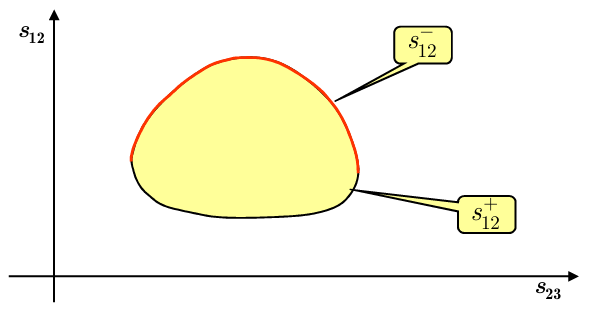
\includegraphics[width=0.8\textwidth]{Lezioni/Lezione 12/tg.png}
    \label{fig:tg}
\end{figure}
Il risultato ottenuto è importante per il Dalitz Plot. Ricordiamo le relazioni
$$
E_1 = \frac{s + m_1^2 - s_{23}}{2\sqrt{s}} \qquad E_2 = \frac{s + m_2^2 - s_{31}}{2\sqrt{s}} \qquad E_3 = \frac{s + m_3^2 - s_{12}}{2\sqrt{s}}
$$
Da esse segue che $dE_1=-2m_nds_{23}$ e le relazioni ottenute da sostituzioni cicliche degli indici:
$$
d\Gamma = \frac{1}{2m_A} |\mathfrak{M}|^2 d\Phi_n \qquad d\Phi = \frac{1}{(2\pi)^3} \frac{1}{4} dE_e dE_\nu \qquad \frac{d\Gamma}{dE_e dE_\nu} = \frac{1}{2m_A} \frac{|\mathfrak{M}|^2}{4(2\pi)^3}
$$
Implicano che la misura di $d\Gamma/dE_1dE_2$ è una misura di $|\mathfrak{M}|^2$: se l'elemento di matrice costante, lo spazio nel piano $E_1-E_2$ (o equiv. $s_{12}-s_{23}$) è popolato uniformemente. Deviazioni dall'uniformità danno indicazioni sulla dipendenza di $|\mathfrak{M}|^2$ dalle variabili $E_1-E_2$
\section{Approssimazione non relativistica}
Ricordiamo l'espressione dell'ampiezza invariante Quindi, ricordiamo l'espressione che avevamo scritto della nostra ampiezza invariante. Allora, settimana scorsa avevamo visto che poi alla fine quello che rimanevano erano gli elementi di matrici delle due correnti, quindi eravamo partiti dalle correnti come operatori di campo nello spazio di Fock, avevamo calcolato gli elementi di matrice fra lo stato iniziale e lo stato finale per la corrente adronica e per la corrente leptonica e avevamo visto che corrispondevano a queste due funzioni che sono quindi le correnti sotto forma a questo punto solo di spinori, non ci sono più gli operatori di campo 
$$
\mathfrak{M} = -iG \overline{u}_{p_p} \gamma^\mu u_{p_n} \overline{u}_{p_e} \gamma_\mu v_{p_\nu}
$$
Concentriamoci sulla parte relativa ai nucleoni (corrente adronica). Nella rappresentazione di Dirac (a bassa energia questa rappresentazione è particolarmente utile) lo spinore del protone è
$$
u_p = \sqrt{E_p + m_p} \begin{pmatrix} \chi^s \\ \frac{\boldsymbol{\sigma} \cdot \mathbf{p}}{E_p + m_p} \chi^s \end{pmatrix}
$$
Analogamente per lo spinore del neutrone. Ricordiamo l'approssimazione non relativistica nella rappresentazione scelta
$$
E_p \approx m_p \qquad \frac{\mathbf{p}}{m_p} \approx 0 \qquad u_p \approx \sqrt{2m_p} \begin{pmatrix} \chi^s \\ 0 \end{pmatrix}
$$
Pertanto
$$
\gamma^0 = \begin{pmatrix} I & 0 \\ 0 & -I \end{pmatrix} \qquad \boldsymbol{\gamma} = \begin{pmatrix} 0 & \boldsymbol{\sigma} \\ -\boldsymbol{\sigma} & 0 \end{pmatrix} \qquad \overline{u}_p = \sqrt{2m_p} (\chi^{\dagger s} \quad 0) \begin{pmatrix} I & 0 \\ 0 & -I \end{pmatrix} = \sqrt{2m_p} (\chi^{\dagger s} \quad 0)
$$
Per la componente temporale della corrente adronica otteniamo pertanto ($m_p\approx m_n\approx m_N$)
$$
\overline{u}_p \gamma^0 u_n = \sqrt{2m_p} \sqrt{2m_n} (\chi^{\dagger r} \quad 0) \begin{pmatrix} \chi^s \\ 0 \end{pmatrix} = 2m_N \chi^{\dagger r} \chi^s = 2m_N \delta_{rs}
$$
Per le componenti spaziali della corrente adronica (gli indici $r$ ed $s$ riguardano la polarizzazione -due qualsiasi polarizzazioni- )
$$
\overline{u}_p \boldsymbol{\gamma} u_n = \sqrt{2m_p}\sqrt{2m_n} (\chi^{\dagger r} \quad 0) \begin{pmatrix} 0 & \boldsymbol{\sigma} \\ -\boldsymbol{\sigma} & 0 \end{pmatrix} \begin{pmatrix} \chi^r \\ 0 \end{pmatrix} = \sqrt{2m_p}\sqrt{2m_n} (\chi^{\dagger r} \quad 0) \begin{pmatrix} 0 \\ -\boldsymbol{\sigma}\chi^r \end{pmatrix} = 0
$$
Vediamo che per $\mu=1,2,3$ le matrici $\gamma^\mu$ mescolano le componenti "large" e "small" degli spinori e pertanto, nell'approssimazione non relativistica danno contributo nullo
$$
\overline{u}_p \gamma^\mu u_n \approx \begin{cases} 2m_N \chi^{\dagger s} \chi^r = 2m_N \delta_{rs} & \mu = 0 \\ 0 & \mu \neq 0 \end{cases}
$$
Il risultato implica che la interazione di Fermi (vettoriale) non prevede che lo spin del nucleone (o del nucleo) non possa cambiare. Nello studio del decadimento $\beta$ furuno presto trovati nuclei che decadevano con variazione dello spin nucleare ad esempio:
$$
\begin{aligned}
\text{He}^6 \, (0^+) &\to Li^6 \, (1^+) + e^- + \overline{\nu} \\
B^{12} \, (1^+) &\to C^{12} \, (0^+) + e^- + \overline{\nu}
\end{aligned}
$$
Divenne pertanto presto chiaro che l'interazione vettoriale doveva essere generalizzata per descrivere anche cambiamenti con variazione dello spin nucleare.
\section{Generalizzazione della Teoria di Fermi}
La scelta di interazione fra correnti vettoriali è solo una delle varie possibili. La richiesta importante da soddisfare è che l'Hamiltoniana sia uno scalare nel senso di Lorentz quindi una quantità costruita come il prodotto di due quadrivettori. Richiesta molto forte che deve essere rispettata ma il prodotto di due quadrivettori non è l'unico modo per ottenere l'invarianza sotto trasformazione di Lorentz. 
$$
\mathcal{H}' = G (\overline{\psi}_p \gamma^\mu \psi_n) (\overline{\psi}_e \gamma_\mu \psi_\nu) + h.c.
$$
L'interazione di Fermi è il prodotto scalare di due correnti vettoriali. Si può generalizzare l'interazione introducendo altre matrici nel vertice di interazione. Quindi mettiamo tra i due spinori altre matrici quadridimensionale che garantiscono comunque che il risultato sia una grandezza scalare.
$$
\mathcal{H}' = G \sum_{i=S,V,A,T,P} C_i (\overline{\psi}_p \Gamma^i \psi_n) (\overline{\psi}_e \Gamma_i \psi_\nu) + h.c.
$$
Le matrici $\Gamma_i$ sono le seguenti combinazioni di matrici $\gamma$ che hanno ben precise proprietà di trasformazione nelle trasformazioni di Lorentz:
\begin{itemize}
    \item $\Gamma_S=1$ Scalare (1 matrice). Questo tipo di accoppiamento viene chiamato scalare perché il termine è la matrice identità
    \item $\Gamma_V=\gamma^\mu$ Vettore (4 matrici) Questo lo abbiamo già visto!
    \item $\Gamma_A=\gamma^5\gamma^\mu$ Vettore Assiale (4 matrici) Un'altra possibilità è un vettore assiale è un quadrivettore che vedremo in dettaglio ma che per definizione risulta proveniente da un prodotto scalare tra due vettori polari in tre dimensioni. Se inverto la direzione degli assi questi vettori assiali rimangono uguali.
    \item $\Gamma_T=\sigma^{\mu\nu}=i/2[\gamma^\mu,\gamma^\nu]$ Tensore (6 matrici)
    \item $\Gamma_P=\gamma^5$ Pseudoscalare (1 matrice).
\end{itemize}
In totale sono 16 matrici indipendenti. Studieremo in seguito il perché di queste denominazioni. Verifichiamo che questa generalizzazione permette anche le variazioni dello spin nucleare. Come nel caso vettoriale utilizziamo la rappresentazione di Dirac. Ricordiamo anche la matrice $\gamma^5$
$$
\gamma^5 = i\gamma^0\gamma^1\gamma^2\gamma^3 = \begin{pmatrix} 0 & I \\ I & 0 \end{pmatrix}
$$
Interazione scalare $\Gamma_S=I$
$$
\overline{u}_p \Gamma_S u_n = \overline{u}_p I u_n \approx \sqrt{4m_p m_n} (\chi^{\dagger s} \quad 0) \gamma^0 I \begin{pmatrix} \chi^r \\ 0 \end{pmatrix} = \sqrt{4m_p m_n} \chi^{\dagger s} \chi^r
$$
Gli spinori $\chi_r$ e $\chi_s$ rappresentano gli stati di spin del nucelone prima e dopo il decadimento. Otteniamo pertanto $(m_p\approx m_n\approx m_N)$
$$
\overline{u}_p u_n \approx 2m_N \chi^{\dagger s} \chi^r = 2m_N \delta_{sr}
$$
Come nel caso vettoriale l'interazione scalare non permette variazioni di spin. Per quanto riguarda invece l'Interazione Vettoriale Assiale
$$
\Gamma_A = \gamma^5 \gamma^\mu
$$
Scriviamo esplicitamente le $4$ matrici $\Gamma_A$
$$
\gamma^5 \gamma^0 = \begin{pmatrix} 0 & I \\ I & 0 \end{pmatrix} \begin{pmatrix} I & 0 \\ 0 & -I \end{pmatrix} = \begin{pmatrix} 0 & -I \\ I & 0 \end{pmatrix}
$$
$$
\gamma^5 \boldsymbol{\gamma}^i = \begin{pmatrix} 0 & I \\ I & 0 \end{pmatrix} \begin{pmatrix} 0 & \boldsymbol{\sigma}^i \\ -\boldsymbol{\sigma}^i & 0 \end{pmatrix} = \begin{pmatrix} -\boldsymbol{\sigma}^i & 0 \\ 0 & \boldsymbol{\sigma}^i \end{pmatrix}
$$
Possiamo subito notare che adesso la matrice $\gamma^5\gamma^0$ mescola componenti large e small al contrario delle matrici $\gamma^5\gamma^i$. Calcoliamo innanzitutto la componente temporale corrente adronica
\begin{align*}
\overline{u}_p \gamma^5 \gamma^0 u_n &\approx 2m_N (\chi^{\dagger s}, 0) \gamma^5 \gamma^0 \begin{pmatrix} \chi^r \\ 0 \end{pmatrix} \\
&= 2m_N (\chi^{\dagger s}, 0) \begin{pmatrix} 0 & -I \\ I & 0 \end{pmatrix} \begin{pmatrix} \chi^r \\ 0 \end{pmatrix} = 2m_N (\chi^{\dagger s}, 0) \begin{pmatrix} 0 \\ \chi^r \end{pmatrix} = 0
\end{align*}
Per quanto riguarda invece le componenti spaziali della corrente adronica
\begin{align*}
\overline{u}_p \gamma^5 \boldsymbol{\gamma}^i u_n &\approx 2m_N (\chi^{\dagger s}, 0) \gamma^5 \boldsymbol{\gamma}^i \begin{pmatrix} \chi^r \\ 0 \end{pmatrix} = 2m_N (\chi^{\dagger s}, 0) \begin{pmatrix} -\sigma^i & 0 \\ 0 & \sigma^i \end{pmatrix} \begin{pmatrix} \chi^r \\ 0 \end{pmatrix} \\
&= 2m_N (\chi^{\dagger s}, 0) \begin{pmatrix} -{\sigma}^i \chi^r \\ 0 \end{pmatrix} = -2m_N \chi^{\dagger s} \sigma^i \chi^r
\end{align*}
In conclusione
$$
\overline{u}_p \gamma^5 \gamma^\mu u_n \approx \begin{cases} 0 & \mu = 0 \\ -2m_N \chi^{\dagger s} \boldsymbol{\sigma}^\mu \chi^r & \mu \neq 0 \end{cases}
$$
Vediamo pertanto che l'Interazione Assiale permette transizioni nucleari con variazione dello spin. Ora per l'Interazione Tensoriale
$$
\Gamma_T = \begin{cases} 0 & \mu = \nu \\ i\gamma^\mu\gamma^\nu & \mu \neq \nu \end{cases}
$$
Iniziamo con le $3$ matrici $\sigma^{0k}$ con $k=1,3$
$$
\sigma^{0k} = i\gamma^0\gamma^k = i \begin{pmatrix} I & 0 \\ 0 & -I \end{pmatrix} \begin{pmatrix} 0 & {\sigma}^i \\ -{\sigma}^i & 0 \end{pmatrix} = i \begin{pmatrix} 0 & {\sigma}^k \\ {\sigma}^k & 0 \end{pmatrix}
$$
Queste matrici mescolano componenti large e small e pertanto $\overline{u}_p\sigma^{0k}u_n\approx0$. Consideriamo adesso le restanti $3$ matrici $\sigma^{kl}$ con $k,l=1,3\,\,\,k\not=l$. Abbiamo già visto che (con $k,l,m$ ciclici e $k,l,m=1,3$)
$$
\sigma^{k,l} = \Sigma^m \qquad \Sigma^m = \begin{pmatrix} {\sigma}^m & 0 \\ 0 & {\sigma}^m \end{pmatrix}
$$
Otteniamo pertanto un risultato analogo a quello dell'interazione assiale
$$
\overline{u}_p \sigma^{\mu\nu} u_n \approx \begin{cases} 0 & \mu \text{ o } \nu = 0 \\ 2m_N \chi^{\dagger s} {\sigma}^m \chi^r & \mu, \nu = 1, 3 \end{cases}
$$
L'interazione Tensoriale permette transizioni nucleari con variazione dello spin. Per finire calcoliamo l'elemento di matrice della corrente adronica per l'Interazione Pseudoscalare
$$
\Gamma_P=\gamma^5
$$
Ricordiamo la forma della matrice $\gamma^5$ nella rappresentazione di Pauli-Dirac
$$
\gamma^5 = i\gamma^0\gamma^1\gamma^2\gamma^3 = \begin{pmatrix} 0 & I \\ I & 0 \end{pmatrix}
$$
La matrice $\gamma^5$ chiaramente mescola le componenti large e small. Pertanto, nell'approssimazione non relativistica
$$
\overline{u}_p \gamma^5 u_n \approx 0
$$
Pertanto nell'Interazione Pseudoscalare, nell'approssimazione non relativistica, non può contribuire al decadimento $\beta$. Riassumendo, la parte relativa ai nucleoni dell'elemento di matrice nella approssimazione non relativistica o "statica" si può approssimare così
\begin{tabular}{|c|c|c|c|}
\hline
% --- Riga Intestazione 1 ---
\multirow{2}{*}{\textbf{Accoppiamento}} & \multicolumn{2}{c|}{\textbf{Elemento di Matrice Nucleare}} & \multirow{2}{*}{} \\
\cline{2-3}
% --- Riga Intestazione 2 ---
& \textbf{Forma covariante} & \textbf{Approssimazione Statica} & \\
\hline
% --- Riga S ---
\textbf{S} & $\overline{u}_p u_n$ & $2m_N \chi^{\dagger s} \chi^r$ & \\
\hline
% --- Riga V ---
\textbf{V} & $\overline{u}_p \gamma^\mu u_n$ & $2m_N \chi^{\dagger s} \chi^r$ & $\mu = 0$ \\
\hline
% --- Riga A ---
\textbf{A} & $\overline{u}_p \gamma^5 \gamma^k u_n$ & $2m_N \chi^{\dagger s} \sigma^k \chi^r$ & $k \neq 0$ \\
\hline
% --- Riga T ---
\textbf{T} & $\overline{u}_p \sigma^{\mu\nu} u_n$ & $2m_N \chi^{\dagger s} \sigma^k \chi^r$ & $\mu,\nu \neq 0$ $k \text{ cyclic}$ \\
\hline
% --- Riga P ---
\textbf{P} & $\overline{u}_p \gamma^5 u_n$ & $\mathbf{0}$ & \\
\hline
\end{tabular}
\subsection{Elemento di matrice nucleare}
La parte relativa al nucleone deve essere feneralizzata per tenere conto del fatto che, in generale, il nucleone è in uno stato legato nel nucleo.
$$
\overline{u}_p \Gamma_X u_n \to \langle X \rangle \equiv \langle N^A_{Z+1} | \hat{O} | N^A_Z \rangle
$$
Gli stati $| N^A_Z \rangle$ e $| N^A_{Z+1} \rangle$ sono rispettivamente le funzioni d'onda iniziale e finale del nucleo. L'operatore $O$ permette un elemento di matrice non nullo fra nuclei diversi: distrugge un neutrone nello stato iniziale e crea un protone nello stato finale. L'operatore $\Gamma$ è una delle matrici introdotte e determina la variaizone di spin. Gli elementi di matrice nucleare sono di due tipi e vengono indicati
$$
\langle 1 \rangle \equiv \langle N^A_{Z+1} | \hat{1} \hat{O} | N^A_Z \rangle \qquad \langle \boldsymbol{\sigma} \rangle \equiv \langle N^A_{Z+1} | \hat{\boldsymbol{\sigma}} \hat{O} | N^A_Z \rangle \qquad 3 \begin{cases} \sigma_x \\ \sigma_y \\ \sigma_y \end{cases}
$$
Il calcolo di questa parte dell'elemento di matrice deve tenere conto della struttura nucleare del particolare nucleo in esame. Non ci occuperemo di questa parte del calcolo.
\section{Generalizzazione dell Teoria di Fermi II}
Dal momento che l'interazione è
$$
\mathcal{H}'_I = G \sum_{i=S,V,A,T} C_i (\overline{\psi}_p \Gamma^i \psi_n) (\overline{\psi}_e \Gamma_i \psi_\nu) + h.c.
$$
L'ampiezza invariante ha 4 termini
$$
\mathfrak{M} = \mathfrak{M}_S + \mathfrak{M}_V + \mathfrak{M}_A + \mathfrak{M}_T
$$
Ricordando quanto detto per l'elemento di matrice nucleare abbiamo:
\begin{itemize}
    \item Scalare
    $$
    \mathfrak{M}_S = G C_S \langle 1 \rangle \overline{u}_e(k) v_\nu(k')
    $$
    \item Vettoriale
    $$
    \mathfrak{M}_V = G C_V \langle 1 \rangle \overline{u}_e(k) \gamma^0 v_\nu(k')
    $$
    \item Vettoriale Assiale (somma di $3$ termini ($j=1,2,3$))
    $$
    \mathfrak{M}_A = G C_A \langle \sigma_j \rangle \overline{u}_e(k) \gamma^5 \gamma^j v_\nu(k')
    $$
    \item Tensoriale nella somma tensoriale ci sono 6 termini (quindi il fattore 2)
    $$
    \mathfrak{M}_T = 2 G C_T \langle \sigma_j \rangle \overline{u}_e(k) \Sigma^{j} v_\nu(k')
    $$
\end{itemize}
Riassumendo: 
\begin{itemize}
    \item Gli accoppiamenti di tipo $S$ e $V$ non possono variare lo spin del nucleone e sono dette Transizioni di Fermi.
    \item Gli accoppiamenti di tipo $A$ e $T$ possono variare lo spin del nucleone e sono dette Transizioni di Gamow-Teller.
    \item Gli accoppiamenti di tipo $P$ si annullano nel limite statico
\end{itemize}
Regole di selezione: 
\begin{itemize}
    \item Transizioni nucleari con $J_i=J_f=0$ sono dette Transizioni Pure di Fermi e possono coinvolgere solo le ampiezze $\mathfrak{M}_S$ e $\mathfrak{M}_V$
    $$
    O^{14} \, (0^+) \to N^{14*} \, (0^+) + e^+ + \nu
    $$  
    \item Transizioni nucleari con $\Delta J=|J_i-J_f|=1$ sono dette Transizioni Pure di Gamow-Teller e possono coinvolgere solo le ampiezze $\mathfrak{M}_A$ e $\mathfrak{M}_T$
    $$
    B^{12} \, (1^+) \to C^{12*} \, (0^+) + e^- + \overline{\nu}
    $$
    \item Transizioni nucleari con $J_i=J_f$ ma con $J_i,J_f\not=0$ sono dette transizioni Miste e possono coinvolgere tutte le ampiezze: $\mathfrak{M}_S$, $\mathfrak{M}_V$, $\mathfrak{M}_A$, $\mathfrak{M}_T$
    $$
    \begin{aligned}
    H^3 &\to He^3 + e^- + \overline{\nu} \\
    n &\to p + e^- + \overline{\nu}
    \end{aligned}
    $$
\end{itemize}
\section{La Larghezza di Decadimento}
Per circa 20 anni l'attività sperimentale fu molto intensa per cercare di capire quali dei possibili accoppiamenti fossero effettivamente realizzati in natura. L'osservabile sperimentale più semplice è lo spettro di energia dell'elettrone. La larghezza di decadimento è data da:
$$
d\Gamma = \frac{1}{2m_n} |\mathfrak{M}|^2 d\Phi
$$
L'elemento dello spazio delle fasi
$$
d\Phi = \frac{d^3 k}{(2\pi)^3 2E_k} \frac{d^3 k'}{(2\pi)^3 2E_{k'}} \frac{d^3 p}{(2\pi)^3 2E_p} (2\pi)^4 \delta^4(P - k - k' - p)
$$
L'elemento di matrice $\mathfrak{M}$ possiede degli indici che identificano gli stati di polarizzazione iniziale e finale delle particelle $\to\mathfrak{M}_{s_i,s_1,s_2,s_3}$. Sappiamo che se non si osserva lo stato di polarizzazione finale occorre sommare i corrispondenti elementi $|\mathfrak{M}|^2$ (somma su $s_1,s_2,s_3$). Se lo stato iniziale non è polarizzato occorre mediare sulle polarizzazioni possibili dello stato inziale (somma su $s_i$). Se non si osservano effetti di polarizzazione si definisce pertanto
$$
\overline{|\mathfrak{M}|^2} = \frac{1}{2} \sum_{s_i=1}^2 \sum_{s_1, s_2, s_3=1}^2 |\mathfrak{M}_{s_i, s_1, s_2, s_3}|^2
$$
\section{Termini di Interferenza}
Il modulo quadrato dell'elemento di matrice contiene termini di interferenza
$$
\overline{|\mathfrak{M}|^2} = \frac{1}{2} \sum_s \mathfrak{M}_s^* \mathfrak{M}_s = \frac{1}{2} \sum (\mathfrak{M}_S^* \mathfrak{M}_S + \dots + \mathfrak{M}_S^* \mathfrak{M}_A + \dots)
$$
L'indice $s$ rappresenta tutti gli indici di spin. Per brevità si è indicato solo un termine di interferenza ($SA$) senza indici $s$. Dimostriamo che i termini di interferenza $SA$, $ST$, $VA$, $VT$ si annullano. Per tutti i termini sopra indicati la parte relativa all'elemento di matrice nucleare contiene termini del tipo $\langle\mathbf{1}\rangle$ e $\langle\boldsymbol {\sigma}\rangle$. Pertanto, trascurando costanti non essenziali (visto che il risultato sappiamo già essere nullo)
$$
\langle 1 \rangle^* \langle \sigma^j \rangle = (\chi^{\dagger s} \chi^r) \chi^{\dagger s} \sigma^j \chi^r = \chi^{\dagger r} \chi^s \chi^{\dagger s} \sigma^j \chi^r
$$
L'indice $j$ si satura con l'indice leptonico corrispondente. Utilizziamo la rappresentazione esplicita per gli spinori di Pauli
$$
\chi^1 = \begin{pmatrix} 1 \\ 0 \end{pmatrix} \qquad \chi^2 = \begin{pmatrix} 0 \\ 1 \end{pmatrix} \qquad \chi_k^s = \delta_{s,k}
$$
Inseriamo nell'espressione del termine di interferenza
$$
\chi^{\dagger r} \chi^s \chi^{\dagger s} \sigma^j \chi^r = \sum_k \chi_k^{\dagger r} \chi_k^s \sum_{l,m} \chi_l^{\dagger s} \sigma^j_{l,m} \chi_m^r
$$
Sommiamo sugli indici di polarizzazione iniziale e finale
$$
\sum_{s,r} \left( \sum_k \chi_k^{\dagger r} \chi_k^s \sum_{l,m} \chi_l^{\dagger s} \sigma^j_{l,m} \chi_m^r \right) = \sum_{s,r} \left( \sum_k \delta_{k,r} \delta_{k,s} \sum_{l,m} \delta_{l,s} \sigma^j_{l,m} \delta_{r,m} \right) = \sum_{s,r} \delta_{s,r} \sigma^j_{s,r}
$$
Pertanto otteniamo in definitiva
$$
\sum_{r,s} \langle 1 \rangle^* \langle \sigma^j \rangle = \sum_{s,r} \delta_{s,r} \sigma^j_{s,r} = \sum_r \sigma^j_{rr} = Tr\sigma^j = 0
$$
Pertanto i termini di interferenza fra elementi di matrice di Fermi e di Gamov-Teller si annullano se mediati sugli stati di polarizzazione. Di conseguenza il quadrato (mediato) dell'ampiezza invariante diventa
$$
\overline{|\mathfrak{M}_S + \mathfrak{M}_V + \mathfrak{M}_A + \mathfrak{M}_T|^2} = \overline{|\mathfrak{M}_S + \mathfrak{M}_V|^2} + \overline{|\mathfrak{M}_A + \mathfrak{M}_T|^2} \equiv \overline{|\mathfrak{M}_F|^2} + \overline{|\mathfrak{M}_{GT}|^2}
$$
Il risultato appena ottenuto permette di semplificare il calcolo: sottolineiamo che succede solo se si media sugli stati di polarizzazione per questo motivo i calcoli per osservabili che dipendono dalla polarizzazione sono un po' più lunghi.
\section{Somme sugli stati di polarizzazione nucleari}
Valutiamo adesso i termini restanti negli elementi di matrice nucleari. Consideriamo ad esempio l'elemento di matrice per una transizione di Fermi
$$
\overline{|\mathfrak{M}_F|^2} = \mathfrak{M}_S^* \mathfrak{M}_S + \mathfrak{M}_V^* \mathfrak{M}_V + 2 \text{Re} \mathfrak{M}_S^* \mathfrak{M}_V
$$
In tutti e tre i termini compare la somma sulle polarizzazioni di termini
$$
\overline{\mathfrak{M}^* \mathfrak{M}} \propto (\overline{u}_p \Gamma^a u_n)^\dagger (\overline{u}_p \Gamma^b u_n)
$$
Abbiamo indicato la matrice genericamente $\Gamma$ perchè considerazioni identiche valgono per le transizioni di Gamow-Teller. Utilizziamo sempre l'approssimazione non-relativistica
$$
u_n \approx \sqrt{2m_N} \begin{pmatrix} \chi^s \\ 0 \end{pmatrix}
$$
La parte dell'elemento di matrice dovuta agli spinori degli adroni è
$$
\overline{\mathfrak{M}^* \mathfrak{M}} \to 4m_N^2 \sum_{rs} (\chi^{\dagger s} \Gamma^a \chi^r)^\dagger (\chi^{\dagger s} \Gamma^b \chi^r) = 4m_N^2 \sum_{rs} (\chi^{\dagger r} \Gamma^{a\dagger} \chi^s) (\chi^{\dagger s} \Gamma^b \chi^r)
$$
Con l'approssimazione non relativistica utilizzata vale $\Gamma^\dagger=\Gamma$ e $\chi^\dagger=\chi^{T}$. Per finire utilizziamo esplicitamente gli indici matriciali nell'espressione
$$
\overline{\mathfrak{M}^* \mathfrak{M}} \propto 4m_N^2 \sum_{r,s} \sum_{jk} (\chi_j^{\dagger r} \Gamma^a_{jk} \chi_k^s) \sum_{lm} (\chi_l^{\dagger s} \Gamma^b_{lm} \chi_m^r)
$$
Ancora una volta utilizziamo la forma esplicita per gli spinori $\chi_k^s=\delta_{s,k}$
$$
\overline{\mathfrak{M}^* \mathfrak{M}} \propto 4m_N^2 \sum_{r,s} \sum_{jk} (\delta_{rj} \Gamma^a_{jk} \delta_{sk}) \sum_{lm} (\delta_{sl} \Gamma^b_{lm} \delta_{rm}) = 4m_N^2 \sum_{r,s} \Gamma^a_{rs} \Gamma^b_{sr} = 4m_N^2 Tr[\Gamma^a \Gamma^b]
$$
Concludiamo il calcolo considerando esplicitamente i due casi:
\begin{itemize}
    \item Transizioni di Fermi (la matrice $\Gamma$ è semplicemente la matrice $I$)
    $$
    \overline{\mathfrak{M}^* \mathfrak{M}} \propto 4m_N^2 Tr[I] = 8m_N^2
    $$
    \item Transizioni di Gamov-Teller (le matrici $\Gamma^a$ sono le matrici di Pauli)
    $$
    \overline{\mathfrak{M}^* \mathfrak{M}} \propto 4m_N^2 Tr[\sigma^a \sigma^b] = 8m_N^2 \delta_{ab}
    $$
\end{itemize}
\section{Il tensore leptonico}
Per la parte leptonica dell'elemento di matrice non si usano approssimazioni ma si utilizza la teoria di Dirac. Occorre calcolare il modulo quadrato degli elementi di matrice del tipo
$$
\mathfrak{M}_{fi} \propto \overline{u}_{p_e} \Gamma^a v_{p_\nu} \qquad \Gamma^a = \hat{1}, \gamma^\mu, \gamma^5\gamma^\mu, \sigma^{\mu\nu}
$$
Per il calcolo di questi termini si possono utilizzare le tecniche di traccia introdotte precedentemente. Abbiamo però una piccola complicazione per la presenza del termine di interferenza
$$
\overline{|\mathfrak{M}_F|^2} = \overline{|\mathfrak{M}_S|^2} + \overline{|\mathfrak{M}_V|^2} + 2\text{Re}\overline{\mathfrak{M}_S^* \mathfrak{M}_V}
$$
In realtà gli spinori e la loro posizione sono gli stessi in tutti e $3$ i termini. In particolare nel termine di interferenza (ad esempio $SV$)
$$
\overline{\mathfrak{M}_S^* \mathfrak{M}_V} \propto (\overline{u}_{p_e} \hat{1} v_{p_\nu})^\dagger (\overline{u}_{p_e} \gamma^\mu v_{p_\nu}) = (\overline{v}_{p_\nu} \hat{1} u_{p_e}) (\overline{u}_{p_e} \gamma^\mu v_{p_\nu})
$$
Dove vediamo somme sulle polarizzazioni e una sorta di relazioni di completezza. La struttura è la stessa degli altri termini. I vertici sono invece mescolati. Un esempio chairirà più di ogni altra spiegazione
\begin{figure}[h!]
    \centering
    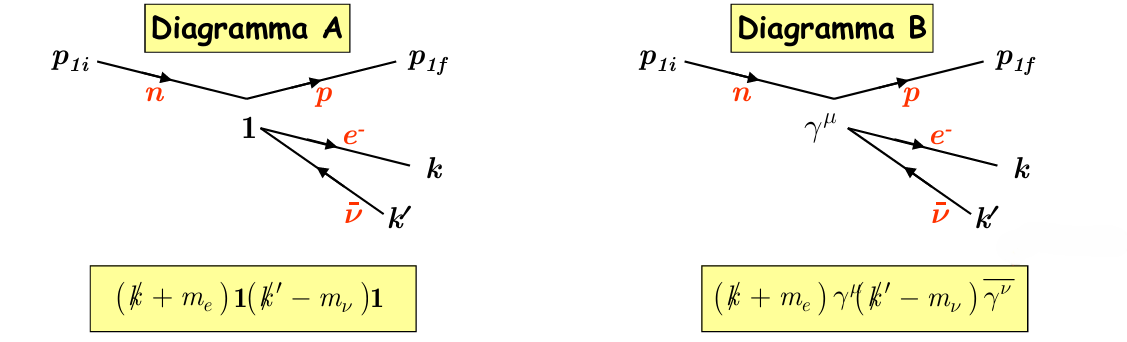
\includegraphics[width=0.9\textwidth]{Lezioni/Lezione 12/poo.png}
    \label{fig:poo}
\end{figure}
Per il Diagramma A per i "quadrati" si introduce nell'ordine: 
\begin{itemize}
    \item Fermione
    \item Vertice
    \item Anti-Fermione
    \item Vertice
\end{itemize}
Per il termine di "interferenza":
\begin{itemize}
    \item Fermione (diagramma A)
    \item Vertice (diagramma A)
    \item Anti-Fermione (diagramma B)
    \item Vertice (diagramma B)
\end{itemize}
\begin{align*}
\overline{|\mathfrak{M}_F|^2} &= C_S^2 4m_N^2 Tr[(\slashed{k} + m_e)(\slashed{k}' - m_\nu)] + C_V^2 4m_N^2 Tr[(\slashed{k} + m_e)\gamma^0 (\slashed{k}' - m_\nu)\gamma^0] + \\
&\quad + 2\text{Re}[C_S C_V 4m_N^2 Tr[(\slashed{k} + m_e)(\slashed{k}' - m_\nu)\gamma^0]]
\end{align*}
\section{L'elemento di Matrice}
Riepilogando, l'elemento di matrice risulta
$$
\overline{|\mathfrak{M}_S + \mathfrak{M}_V + \mathfrak{M}_A + \mathfrak{M}_T|^2} = \overline{|\mathfrak{M}_S + \mathfrak{M}_V|^2} + \overline{|\mathfrak{M}_A + \mathfrak{M}_T|^2} = \overline{|\mathfrak{M}_F|^2} + \overline{|\mathfrak{M}_{GT}|^2}
$$
Calcoliamo il termine relativo alle transizioni di Fermi $\overline{|\mathfrak{M}_F|^2}$
$$
\overline{|\mathfrak{M}_F|^2} = \overline{|\mathfrak{M}_S|^2} + \overline{|\mathfrak{M}_V|^2} + 2 \text{Re} \overline{\mathfrak{M}_S^* \mathfrak{M}_V}
$$
Abbiamo visto che
$$
\mathfrak{M}_S = G C_S \langle 1 \rangle \overline{u}_e(k) v_\nu(k') \qquad \mathfrak{M}_V = G C_V \langle 1 \rangle \overline{u}_e(k) \gamma^0 v_\nu(k')
$$ 
Dove abbiamo anche calcolato $\langle1\rangle=8m_N^2$ e assumento $C_S$ e $C_V$ reali otteniamo
\begin{align*}
\overline{|\mathfrak{M}_F|^2} &= G^2 C_S^2 4m_N^2 Tr[(\slashed{k} + m_e)(\slashed{k}' - m_\nu)] + \\
&\quad + G^2 C_V^2 4m_N^2 Tr[(\slashed{k} + m_e)\gamma^0 (\slashed{k}' - m_\nu)\gamma^0] + \\
&\quad + 2\text{Re}[G^2 C_S C_V 4m_N^2 Tr[(\slashed{k} + m_e)(\slashed{k}' - m_\nu)\gamma^0]]
\end{align*}
Per il momento non indicheremo pià $G^2$ e lo reintrodurremo alla fine del calcolo. Vari conti assolutamente non richiesti si arriva alla forma:
$$
\overline{|\mathfrak{M}_F|^2} = 16m_N^2 E_e E_\nu G^2 \left[ C_S^2 (1 - \boldsymbol{\beta}_e \cdot \boldsymbol{\beta}_\nu) + C_V^2 (1 + \boldsymbol{\beta}_e \cdot \boldsymbol{\beta}_\nu) + 2C_S C_V \frac{m_e}{E_e} \right]
$$
Un calcolo analogo per l'elemento di matrice di Gamov-Teller
$$
\overline{|\mathfrak{M}_{GT}|^2} = 16m_N^2 E_e E_\nu G^2 \left[ 3C_A^2 \left(1 - \frac{1}{3}\boldsymbol{\beta}_e \cdot \boldsymbol{\beta}_\nu\right) + 12C_T^2 \left(1 + \frac{1}{3}\boldsymbol{\beta}_e \cdot \boldsymbol{\beta}_\nu\right) - 12C_A C_T \frac{m_e}{E_e} \right]
$$